\section{Question 1}

\textbf{Which database video does the recorded query match the most?}

\begin{figure}[h] 
\centerline{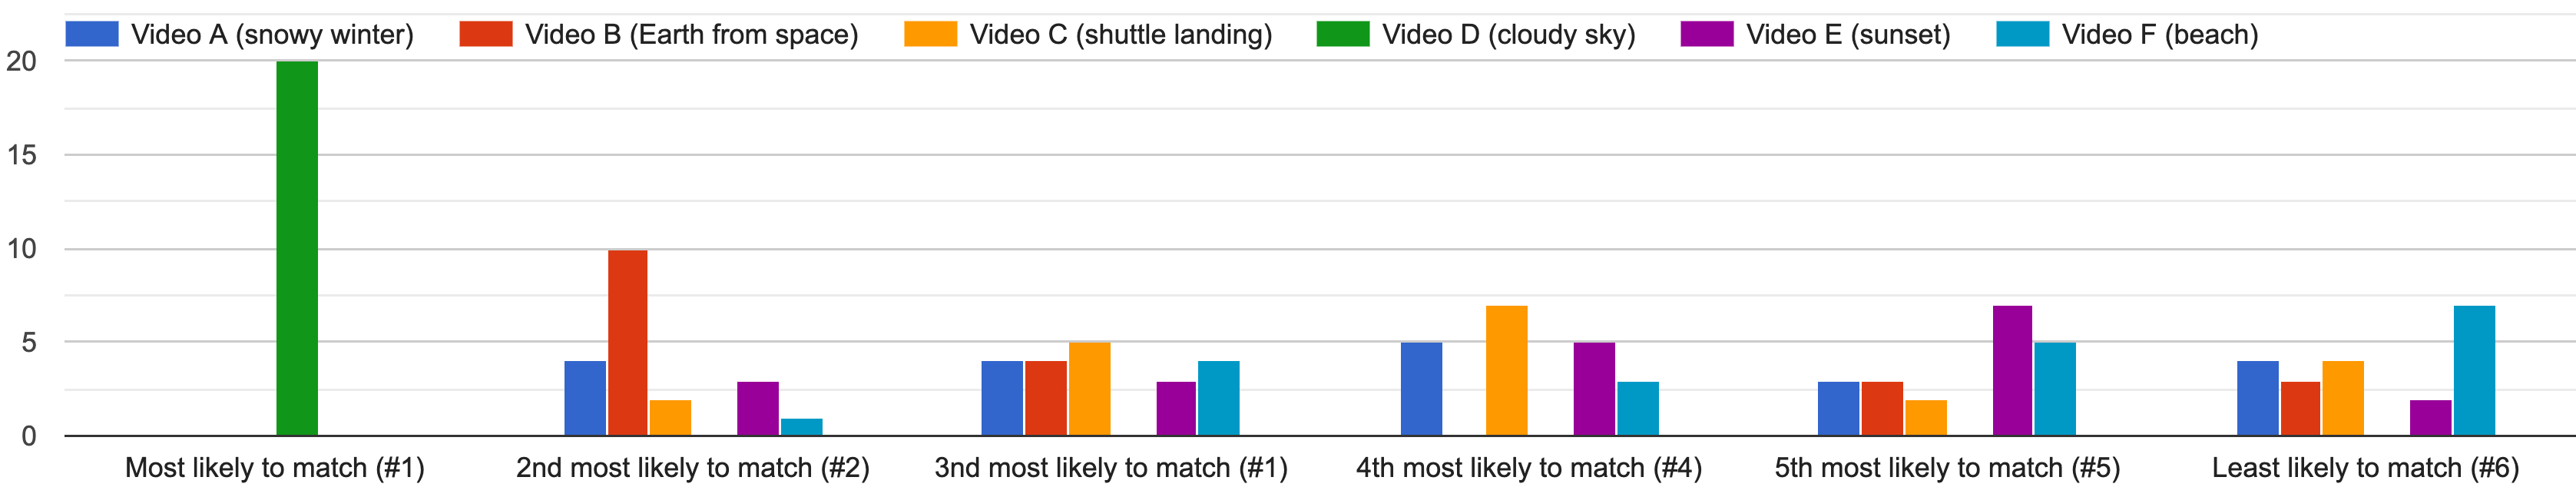
\includegraphics[width=1.1\textwidth]{figures/appendix/survey_results.png}}
\caption{\label{fig:appendix_survey_results}Survey results of the ``Which database video does the recorded query match the most?'' ranking question.}
\end{figure}

\section{Question 2}

\textbf{Which video aspects did you consider the most when ranking them?}

\begin{itemize}
	\item Participant 1: Blue colour
    \item Participant 2: the sky is cold
    \item Participant 3: The colours and movements
    \item Participant 4: The colour of the sky and the movements
    \item Participant 5: Colours and luminosity
    \item Participant 6: The actual scenario i.e. the fact that a plane was landing or the fact that someone was walking a dog
    \item Participant 7: Light, sky and clouds
    \item Participant 8: clouds
    \item Participant 9: colour, landscape, sounds
    \item Participant 10: movement, patterns, image, colour
    \item Participant 11: luminosity of colours and similarity of object represented
    \item Participant 12: Images, absence of sound, speed of movement
    \item Participant 13: Colours
    \item Participant 14: Colour, movement, size of objects, shape of objects
    \item Participant 15: Image, colour, light
    \item Participant 16: The colours (including luminosity) then the movements
    \item Participant 17: colour blue with blurry whites. sky clearly visible in daytime
    \item Participant 18: The movement and colour of the image
    \item Participant 19: Colours
    \item Participant 20: Colours of the video
\end{itemize}

\section{Question 3}

\textbf{What do you think is the most important aspect of a video that a matching algorithm should analyse when pattern matching videos?}

\begin{itemize}
	\item Participant 1: Similar colours, shades of colours
    \item Participant 2: colours (warm vs cold) 
    \item Participant 3: Colours 
    \item Participant 4: Colours and the pace of movement and change
    \item Participant 5: Colours
    \item Participant 6: colour
    \item Participant 7: The environment surrounding the action
    \item Participant 8: overall colour and location of major colour blobs
    \item Participant 9: filter / colours, sounds (as many movies can relate similar situation e.g. Second World War, they can be differentiated by determining how old is the movie and where it takes place). Sounds are very different from one movie to another, even in the same topic, so I believe that it is another core aspect to be analysed.
    \item Participant 10: movement 
    \item Participant 11: shapes and luminosity 
    \item Participant 12: Image + speed of movement 
    \item Participant 13: Colours / Shapes / moving objects
    \item Participant 14: Colour scheme
    \item Participant 15: Sound, quality of image
    \item Participant 16: The motion and the colours
    \item Participant 17: objects appearing in video
    \item Participant 18: The succession of images
    \item Participant 19: movements
    \item Participant 20: Shape and colour of objects within the video
\end{itemize}
